 % Chapter Template

\chapter{Evaluation} % Main chapter title

\label{Chapter6} % Change X to a consecutive number; for referencing this chapter elsewhere, use \ref{ChapterX}

In order to evaluate my work, I compare the architecture and implementation of my prototype with the existing Project EPIC infrastructure along the dimensions of reliability, scalability, performance, and real time delivery.

\section{Reliability}

In order to evaluate my work, I compare the architecture and implementation of my prototype with the existing Project EPIC infrastructure along the dimensions of reliability, scalability, performance, and real-time delivery.

\subsection{Current infrastructure}

Reliability of the existing EPIC infrastructure needs to be studied separately across EPIC Collect and EPIC Analyze.

EPIC Collect is designed to be highly available. It is implemented as a multi-threaded Java application; some threads are used to read the incoming tweet stream, some are used to classify tweets, and some are used to monitor the other threads. If the monitoring threads detect that one of the readers is no longer producing tweets for the classifiers, it can issue a command that causes the current connection to the Twitter Streaming API to be dropped and all of these threads to be deactivated. This action, in turn, causes another thread to detect that the Twitter connection is down and it then restarts the connection which causes readers, classifiers, and monitors to once again be instantiated. This approach can ensure reliable performance for many days; however, sometimes errors occur that cause all threads to lock up. To handle this situation, EPIC Collect makes use of a cron job that wakes up once per minute to examine the current length of the EPIC Collect log file. Each reader and classifier will send information to the log file and when data collection is proceeding smoothly, the log file is always increasing in size. As a result, if the cron job wakes up and discovers that the log file has not increased in size over the past minute, it assumes that the collection software has locked up. It will invoke a command to kill the previously running process and it then invokes the collection system, notes the size of the log file, and goes back to sleep.

With these techniques, EPIC Collect has achieved 99\% uptime since the summer of 2012. The only problem that these techniques cannot account for is if the data center loses its network connection. When that happens, the cron job will be stuck in a cycle of terminating and restarting the software until the network connection is restored. Fortunately, complete loss of the data center’s connection to the Internet is a very rare event, happening only once in a four year period.

EPIC Analyze does not have the same level of reliability.In order for the web application to function, it requires that Redis and Solr be up and running. If these systems are not available, then the web application is non-functional. Compounding this situation is the fact that EPIC Analyze is deployed manually by its developers; there is no automated way to deploy it and there is no monitoring system detecting for system failure. As a result, there is also no automated recovery procedure. All aspects of the system deployment for EPIC Analyze require manual intervention by developers.

\subsection{System Prototype}

In the case of my system prototype, overall reliability is high, due to the use of a container-orchestration system. Kubernetes provides two components to increase the reliability of our system. The first Kubernetes-provided component is the controller manager that runs on the master node of our cluster. This component is responsible for keeping track of all containers running on our cluster. It also follows the requests made by the infrastructure controller to ensure that the right number of replicas are created for the components that need them. For instance, in my prototype, I specify that there should be two replicas of a Kafka broker available at all times. If any of those replicas go down, Kubernetes will detect that and launch a new one. This functionality extends to all of our containers; if any container stops running, the controller manager detects it and schedules a new instance of that container to run on an available node. This check is performed when the infrastructure controller makes new requests or when an existing node informs the controller manager that one of its containers went down.

The second Kubernetes-provided component is the scheduler. This component makes sure that new containers are scheduled on the best node possible. Kubernetes allows an engineer to configure the amount of memory and cpu permitted by a container; this information allows the scheduler to find the best fit for each deployment request.

With these two components, Kubernetes automates the deployment of containers on a cluster of machines and handles any failures automatically. Its services are significantly more advanced than the existing reliability measures put into place by the Project EPIC developers, who were more interested (at the time) in system functionality and not in automated failure recovery mechanisms beyond what was done to ensure reliable data collection.

Kubernetes provides one additional reliability-related feature and that is related to upgrading containers to provide new versions of the microservice within---this feature is called a \textit{rolling update}. When performing an upgrade, the controller manager first deploys the new version of the component and ensures that it is up and running. It then removes the container containing the previous version of the component. I make use of this functionality with the Twitter Tracker component. When a new change to data collection is announced by the Event Manager, the infrastructure controller arranges to have a new instance of the Twitter Tracker component deployed with the new state. It starts to collect tweets using the newly updated keyword list while the previous instance is still collecting data on the prior set of keywords. This approach ensures that no tweets are missed when the transition occurs. Twitter applications can only have one standing connection. When the new instance establishes a connection, Twitter will close the old connection ensuring that there will not be any duplicated tweets stored in the transition.

Figure \ref{fig:pods} displays a typical report for the number of times the containers in our system prototype were restarted automatically by Kubernetes over a period of eleven days with no interaction from the user. The first thing to note is that all components remained active for the entire time period; that is data collection proceeded uninterrupted during those eleven days. However, due to system demands, Kubernetes may have found itself needing to, for instance, delete a container on an overloaded node and move it to a node that had more resources available. Given that my code is now fairly stable, if we increased the amount of memory on each node and added a few more nodes to our cluster, the total number of restarts would go down. But, given the limited resources I had during development, the more important issue is that despite limited resources, the system continued to run 24/7 with no interventions required by the developer.  Note: that in Figure \ref{fig:pods}, some instances are listed as only existing for two days; this discrepancy is due to the fact that Kubernetes will restart a container’s count if it needs to do a hard restart of the container. This occurs when Kubernetes issues a request for the container to shut down and it stays active, ignoring the request. This might occur due to the contained microservice crashing inside and thus unable to exit gracefully. As a result, Kubernetes is forced to kill the container without a graceful shutdown.

\begin{figure}
\centering
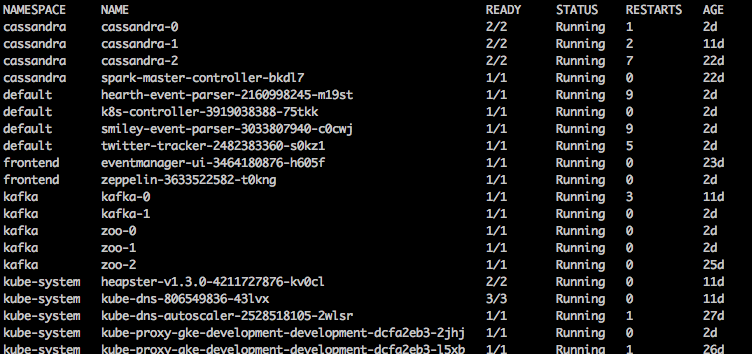
\includegraphics[width=\textwidth]{Figures/pods}
\decoRule
\caption[Kubernets restarts in eleven days]{Number of automated restarts by Kubernetes of the system prototype over a period of eleven days.}
\label{fig:pods}
\end{figure}

\section{Scalability}

The second dimension I am using for my evaluation is scalability. I am interested in how well both infrastructures deal with the ability to scale to large amounts of data. I want to avoid wasting system resources unnecessarily while having the capacity to scale and I want to understand how scaling impacts overall system performance.

\subsection{Current infrastructure}

Scalability with the existing infrastructure is not a straightforward process. With respect to throughput capacity, EPIC Collect would need a developer to manually launch a new instance with new Twitter credentials and set-up a second cron job to monitor the second instance’s log files. That work is feasible but not straightforward and would have to be performed anew if more capacity was needed and a third instance was required. This situation is one reason why EPIC Collect does not perform data normalization; it simply classifies tweets with respect to the current set of events and then it stores them in Cassandra. If data normalization was added to the existing EPIC Collect then it would struggle to handle spikes in incoming traffic as it would not be able to automatically scale its capacity to handle demand.

With respect to storage capacity, EPIC Collect is in a better situation since it stores tweets to a four-node Cassandra cluster with terabytes of disk space available. If additional capacity is needed, a developer just needs to configure a new node and add it to the existing cluster. As with the discussion above concerning throughput capacity, while this works, it is hardly an automated approach to scaling the infrastructure on demand.
With respect to EPIC Analyze, the only component that is a target for scaling, apart from storage, is the frontend module that is currently written in Ruby on Rails. To do that, multiple instances of the application would need to be launched and a load balancer put in front of those instances. To make this work, the existing web application would need to be refactored such that session state can be made consistent across all of the instances. That is a straightforward engineering task but not simple by any means. Furthermore, maintaining a load balancer is a complex process when done manually and, as discussed above, all maintenance on EPIC Analyze has to be performed manually.

I conclude that the existing Project EPIC infrastructure is not easy to scale.

\subsection{System Prototype}

Scaling my system prototype is much easier given the functionality gained from Kubernetes. When deploying a microservice via a container, I can specify how many replicas of that service I would like to deploy alongside it. The controller manager will try to schedule the requested number of replicas as long as there are enough system resources available across the cluster. Our ability to deploy multiple replicas is helped by the fact that most of our services were designed to be stateless. All of the state that a service needs to perform its task is contained in the messages that it receives. As a result, it does not matter which replica handles a given input message. Replicas can also be automatically triggered based on CPU usage. If a container hits 90\% CPU utilization because it has experienced a spike in the number of input messages, Kubernetes can automatically spin up new replicas until the utilization goes down, due to the fact that the new replicas can help the existing component handle the spike in messages.

While these services are largely automatic, a developer can always interact with Kubernetes directly to manually deploy additional components to help with scalability. The developer can issue these commands using the \texttt{kubectl} command line tool or via Kubernetes’s web interface.

Due to the features of container orchestration systems, my system prototype is much easier to scale than the existing Project EPIC infrastructure.

\section{Performance}

I am unable to provide a comparison between the two infrastructures with respect to performance. Both systems have similar performance with respect to data collection but detailed tests and comparisons are not possible since EPIC Collect is a production system that other members of the Project EPIC team depend on for their research. As such, in this section, I provide insight into the performance my system prototype achieves on my small four-node cluster. As a reminder, each node in the cluster has access to one virtual CPU and four gigabytes of RAM. My test involves executing a Spark-based job on the cluster to count the number of words contained in all collected tweets. Each time I ran the query for the evaluation, the total number of tweets collected was different, increasing each time. I selected this particular test since word count is a highly parallelizable operation. It also demonstrates the integration of Spark into my system prototype.

The code entered into Zeppelin is shown in Listing \ref{lst:wordcount}.  The first line establishes a connection to Cassandra and creates a Spark Context object by which queries can be invoked. The second line expresses a series of transformations that Spark will apply to count all of the words of all tweets contained in Cassandra. It starts by selecting the text of the tweet, splitting the text into words, mapping each word into a pair (word, 1) and then reducing all such pairs by adding up the integers for each matching key. Thus all pairs like (cat, 1) would eventually turn into a single pair (cat, 1000) where 1000 represents the number of times that cat appears in the collected tweets. Finally, the pairs are inverted, e.g. (1000, cat), and then sorted in descending order.

The power of Spark is that all of these transformations are applied to every tweet in parallel and, furthermore, as much of the transformations are applied locally on every node before any data is sent to the master node for the final combination of pairs across nodes. Spark provides a mechanism to reveal how it will execute a query known as the debug string.

\begin{lstlisting}[language=scala, caption={WordCount Spark script},float, floatplacement=H, label={lst:wordcount}]
val table = sc.cassandraTable("twitter_analytics", "tweet")
val words = table.select("t_text").flatMap(l => l.getString("t_text").split(" "))
      .map(word => (word.toLowerCase,1)).reduceByKey(_ + _).map(_.swap).sortByKey(false,1)
\end{lstlisting}

Each indentation in the debug string is a map stage, and each `+' is a shuffle phase. As we can see in Listing \ref{lst:rddebug}, Spark delays shuffling data until it is time to execute the \texttt{reduceByKey} step. This makes sense since it can generate word pairs on each node without having to transfer data across nodes. However, once it needs to count the total number of words, it has to send data across nodes to a master node to create the final counts. It then performs one more shuffle when it sorts the final key-value pairs after swapping them from this format (cat, 1000) to this format (1000, cat).

\begin{lstlisting}[language=scala, caption={Debug string rdd}, float, floatplacement=H, label={lst:rddebug}]
(1) ShuffledRDD[112] at sortByKey at <console>:31 []
+-(176) MapPartitionsRDD[111] at map at <console>:31 []
    |   ShuffledRDD[110] at reduceByKey at <console>:31 []
    +-(176) MapPartitionsRDD[109] at map at <console>:31 []
        |   MapPartitionsRDD[108] at flatMap at <console>:31 []
        |   CassandraTableScanRDD[107] at RDD at CassandraRDD.scala:15 []
\end{lstlisting}

As we can see in Figure \ref{fig:wordcountplot},  the word count performance is linear but with a flat slope at the beginning indicating that performance improved with larger numbers of tweets to analyze (see the increase in tweets processed per second in Table \ref{tab:numtweets}) and then increasing as the total size of the data set went past 2M tweets. The likely reason for this performance curve is that there is a certain amount of overhead that is incurred each time to stage the job and perform the shuffle steps at the end, counting up the pairs and sorting them. However, as the number of tweets increases, each individual node can do more work uninterrupted and can execute as quickly as possible without the need for coordination messages. As a result, the performance per tweet increases as the datasets get larger and this keeps performance acceptable.

\begin{figure}
\centering
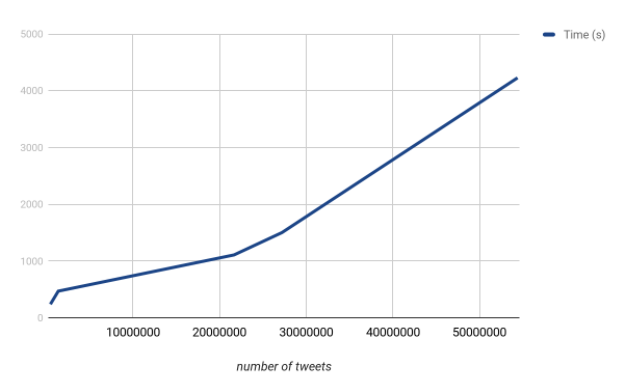
\includegraphics[width=\textwidth]{Figures/wordcountplot}
\decoRule
\caption[Wordcount time plot]{Plot on wordcount time for dataset size}
\label{fig:wordcountplot}
\end{figure}

\begin{table}
\centering
\begin{tabular}{r r r}
\toprule
\textbf{Number of tweets} & \textbf{Time (s)} & \textbf{Tweets/sec}\\
\midrule
490199 & 238 & 2060 \\
1400884 & 469 & 2987 \\
21680851 & 1107 & 19585 \\
27199614 & 1500 & 18133 \\
54395957 & 4228 & 12866 \\
\bottomrule\\
\end{tabular}
\caption{Number of tweets in dataset and performance metrics}
\label{tab:numtweets}
\end{table}

\section{Software development and maintenance}

One of my goals was to develop a system that was easier to maintain. I accomplished this primarily through the use of microservices. The code associated with a microservice is small, making it easier for new developers to understand and maintain it. Furthermore, as was the case with several of our components, we wanted to make it straightforward for a developer to reimplement one of our components if there was a compelling reason to do so, such as poor performance.

\subsection{Current infrastructure}

Currently the code for this infrastructure is split at a high-level into two separate, large and complex projects. This presents challenges to new developers on the Project EPIC team in terms of getting to know the code to a point where they feel confident they can contribute to it.

The Ruby-on-Rails portion of EPIC Analyze has 5086 lines of code and is maintained in a git repository on GitHub. It is thus easy for multiple developers to work on it but it takes a lot of work to understand it. It relies heavily on Ruby-on-Rails conventions and that adds an extra layer of difficulty for developers unfamiliar with that framework. In addition, EPIC Analyze relies on the use of solr and redis, two middleware services that both have significant learning curves. EPIC Collect is likewise a large system, consisting of thousands of lines of Java code that rely heavily on the Spring Framework.\footnote{\href{https://spring.io}{https://spring.io}} Learning that codebase is difficult, even for experienced developers, and requires a sophisticated understanding of a wide range of Java infrastructure: maven, jenkins, Tomcat, and more. Finally, it is difficult to debug changes to both systems: EPIC Analyze requires deploying multiple servers on multiple machines as does EPIC Collect and the latter has additional monitoring software that must be configured and maintained as well. The result is that the current Project EPIC infrastructure is difficult to maintain.

\subsection{System Prototype}

My system prototype is divided into two main parts. The first part consists of the code for the various components, written in both Python and Go. The second part consists of declarative configuration documents written in YAML that specify how to deploy the infrastructure into Kubernetes.\footnote{Yet Another Markup Language}

\begin{itemize}
	\item \textit{Twitter tracker (Go)}: 108 lines
	\item \textit{Kubernetes controller (Python)}: 145 lines
	\item \textit{Event manager (Python/Django)}: 2090 lines
	\item \textit{Tweet normalizer (Python)}: 209 lines
\end{itemize}

The largest component is the Event manager but that is not surprising as it requires all the code that is normally associated with a fully functioning web application. Otherwise, the code is fairly equally distributed among the various microservices. Each service is small and easy to understand. Different developers can work on each microservice and then those services can be linked via Kubernetes and Kafka. Furthermore, due to the use of Kafka, each microservice can be written in a different technology stack allowing us to choose the tools and languages best suited to each task. As long as the technologies that we select can be containerized, then the resulting microsevice can easily be deployed by Kubernetes.

The YAML files consist of 3345 lines of declarations that knit all of the components together. Kubernetes currently requires developers to manually write and review each YAML file but developers are working on new tools that will reduce the need to generate them by hand.

As a result, my system prototype has significantly reduced maintenance costs. It is straightforward to develop simple microservices and then the use of Docker, Google Cloud, and Kubernetes makes it much easier to deploy those services into a production environment that can be scaled on demand.

